\documentclass[a4paper,11pt, titlepage]{extarticle}

\usepackage{amsmath}
\usepackage{amssymb}
\usepackage{blindtext}
\usepackage{caption}
\usepackage{charter}
\usepackage{color}
\usepackage{comment}
\usepackage{empheq}
\usepackage{fancyhdr}
\usepackage[T1]{fontenc}
\usepackage{gensymb}
\usepackage[top=2cm, bottom=2.5cm, left=1.5cm, right=1.5cm, footskip=0.7cm]{geometry}
\usepackage{graphicx}
\usepackage{indentfirst}
\usepackage[utf8]{inputenc}
\usepackage{lastpage}
\usepackage{listings}
\usepackage{pdflscape}
\usepackage{pdfpages}
\usepackage{prftree}
\usepackage{setspace}
\usepackage{subcaption}
\usepackage{titlesec}
\usepackage{tikz}
\usepackage[normalem]{ulem}
\usepackage{verbatim}
\usepackage{wrapfig}

\titleformat{\title}
{\color{black}\normalfont\Large\bfseries\centering}
{\color{black}\thesection}{1em}{\hspace{0cm}}

\titleformat{\section}
{\color{black}\normalfont\LARGE\bfseries}
{\color{black}\thesection}{1em}{\hspace{0cm}}

\titleformat{\subsection}
{\color{black}\normalfont\Large\bfseries}
{\color{black}\hspace{.2cm}\thesubsection}{1em}{\hspace{.3cm}}

\titleformat{\subsubsection}
{\color{black}\normalfont\large\bfseries}
{\color{black}\hspace{.4cm}\thesubsubsection}{1em}{\hspace{.6cm}}

\title{Simulation du trafic routier atours du CERN}
\author{Pavlos Tserevelakis \and Raphaël Lutz}
\date{7 septembre 2018}

\definecolor{codegreen}{rgb}{0,0.6,0}
\definecolor{codegray}{rgb}{0.5,0.5,0.5}
\definecolor{codeblue}{rgb}{0,0,1}
\definecolor{codebordeau}{rgb}{0.5,0.1,0}
\definecolor{backcolour}{rgb}{0.95,0.95,0.95}
 
\lstdefinestyle{mystyle}{
    backgroundcolor=\color{backcolour},   
    commentstyle=\color{codegreen},
    keywordstyle=\bfseries\color{codebordeau},
    numberstyle=\tiny\color{codegray},
    stringstyle=\color{codeblue},
    basicstyle=\footnotesize,
    breakatwhitespace=false,         
    breaklines=true,                 
    captionpos=b,                    
    keepspaces=true,                 
    numbers=left,                    
    numbersep=5pt,                  
    showspaces=false,                
    showstringspaces=false,
    showtabs=false,                  
    tabsize=2
}
 
\lstset{style=mystyle}
\renewcommand{\contentsname}{Table des matières}

\begin{document}

\begin{titlepage}
	\centering
	
\includegraphics[width=0.45\textwidth]{logoUni.jpg}\par
	\vspace{3cm}
	{\Large Étude sur le trafic routier au CERN \par}
	\vspace{1.5cm}
	{\scshape\huge\bfseries Simulation du trafic routier\\autours du CERN\par}
	\vspace{1.5cm}
	{\scshape\Large Pavlos Tserevelakis et Raphaël Lutz\par}
	\vspace{1.5cm}
	{\large\itshape supervisés par Prof. Bastien Chopard et Prof. Pierre Leone (Unige)\\et Frédéric Magnin (CERN)\par}
	\vspace{1.5cm}
	{30 novembre 2018\par}
	\vspace{6.5cm}
	{https://github.com/lutzilutz/TraficCERN\par}
	\vfill
\end{titlepage}

%\maketitle

\tableofcontents\newpage

\begin{comment}\pagestyle{fancy}
\renewcommand{\headheight}{24pt}
\lhead{Pavlos Tserevelakis et Raphaël Lutz}
\rhead{30 novembre 2018}\end{comment}

\section{Présentation de l'étude}

La présente étude, demandée par Frédéric Magnin (directeur du département Civil Engineering and Buildings) pour le CERN, vise à modéliser le réseau routier environnant le CERN afin d'en simuler le trafic et tester différents scénarios possibles pour améliorer la circulation aux abords du CERN, ainsi que de limiter l'impact du personnel du CERN sur la circulation. L'étude a été réalisée dans le cadre du cours \emph{Applications Informatiques} de notre Bachelor en Sciences Informatiques.

\subsection{Scénarios étudiés}

Nous avons étudié les scénarios suivants afin de juger de leur pertinence et de leur impact sur le trafic routier, en accord avec Frédéric Magnin.

\begin{itemize}
\item Scénario actuel
\item Report de véhicules depuis les entrées A et B vers l'entrée E
\item Remplacement du carrefour à feux de l'entrée B par un rond-point
\item Diminution du temps de contrôle à l'entrée E
\end{itemize}

\subsection{Informations complémentaires}

\begin{table}[h!]
\begin{center}
\begin{tabular}{l|c|c}
 & min & max \\ \hline
de l'entrée A vers l'entrée E & 20\% & 50\% \\ \hline
de l'entrée B vers l'entrée E & 30\% & 70\% \\ 
\end{tabular}
\end{center}
\caption{Valeurs utilisées pour le report de véhicules}
\label{tabReport}
\end{table}

Lorsque dans cette étude nous parlerons de ``report minimum'' et ``report maximum'', cela fera référence à ce tableau. Dans le cas du report minimum, 20 et 30\% des véhicules rentrant normalement par les entrées A et B seront redirigés vers l'entrée E. De même pour le report maximum, où ces valeurs seront de 50 et 70\%.

\vspace{0.4cm}

Nous allons également parler de ``scénario 2'', ceci faisant référence au remplacement du carrefour de l'entrée B par un rond-point.

\newpage

\section{Modèle utilisé}

Nous avons choisi d'implémenter un modèle discret du trafic routier, par automate cellulaire. Ce genre de modèle a fait ses preuves, comme présenté par le professeur Bastien Chopard\footnote{\emph{Cellular Automata Simulations of Traffic:
A Model for the City of Geneva}, A. Dupuis et B. Chopard, Networks and Spatial Economics, 3: (2003) 9–21}. Ce genre de modèle est beaucoup plus simple à implémenter qu'un modèle continu, et offre pourtant une très bonne représentation de la circulation : embouteillages, accélération/décélération, effet accordéon, ... Ce choix nous a donc amener à procéder à plusieurs décisions nécessaires.

\subsection{Dimensions}

Nous avons décidé de prendre comme longueur d'une cellule $7,5 \; [m]$. Ceci correspond bien à la longueur moyenne d'un véhicule personnel. Nous décidons aussi de prendre 1 étape de simulation comme 1 seconde. Nous obtenons donc les deux vitesses suivante : $7,5 \; [\frac{m}{s}] = 27 [\frac{km}{h}]$ et $15 \; [\frac{m}{s}] = 54 [\frac{km}{h}]$.

\begin{table}[h!]
\begin{center}
\begin{tabular}{|l|c|c|}
\hline
 & vitesse 1 & vitesse 2 \\ \hline
\#cellule$/s$& 1 & 2 \\ \hline
$m/s$ & 7.5 & 15 \\ \hline\hline
$km/h$ & 27 & 54 \\ \hline
\end{tabular}
\end{center}
\caption{Vitesses choisies}
\label{tabSpeed}
\end{table}

Les véhicules sont limités à ces deux vitesses, résumées dans la table \ref{tabSpeed}.

\subsection{Délimitation du réseau}

\begin{figure}[!h]
  \begin{center}
    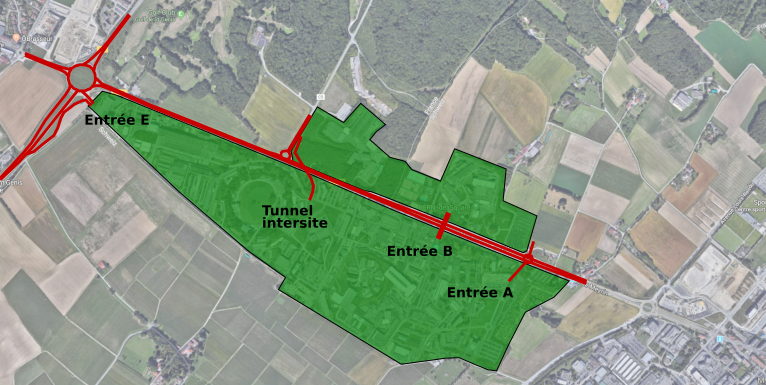
\includegraphics[width=0.7\textwidth]{images/reseauRoutier.png}
  \end{center}
  \vspace{-0.4cm}
  \caption{En rouge les routes intégrées au réseau, en vert les zones du CERN}
  \label{imgReseau}
  \begin{center}
    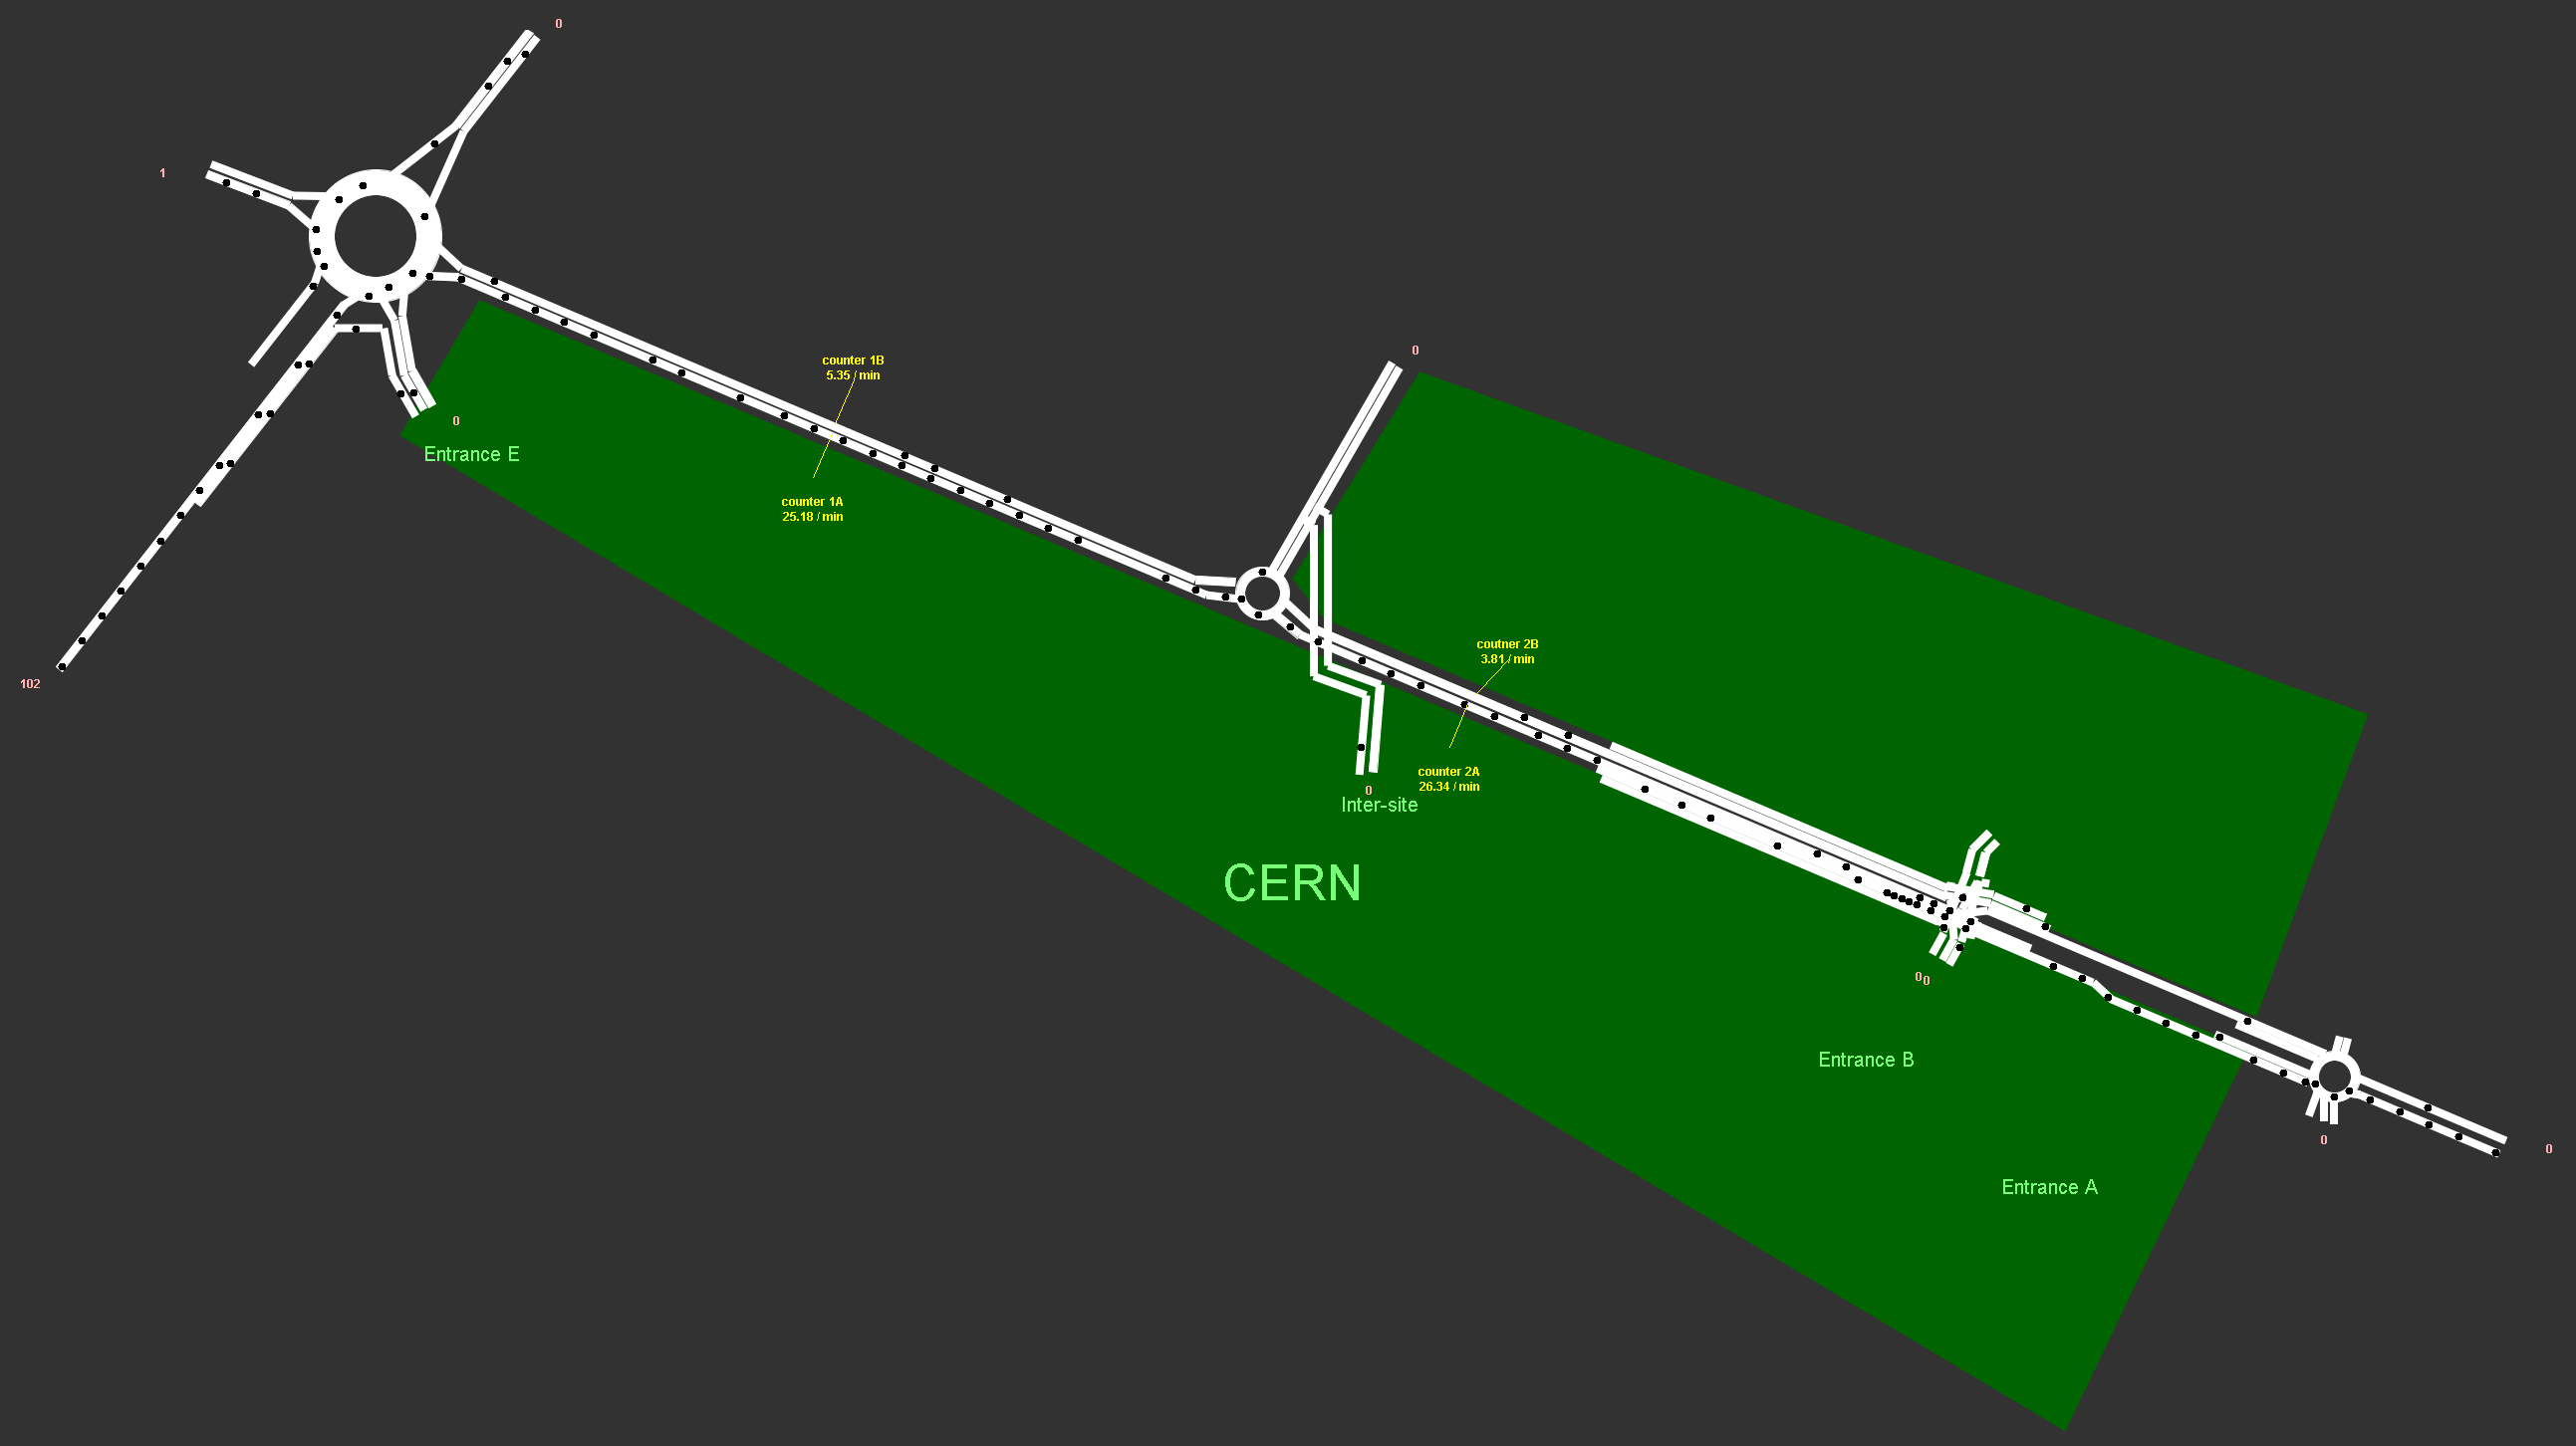
\includegraphics[width=0.7\textwidth]{images/simulateurReseau.png}
  \end{center}
  \vspace{-0.4cm}
  \caption{L'implémentation du réseau dans le simulateur}
  \label{imgReseauSim}
\end{figure}


La modélisation du réseau s'est limité à l'axe routier passant par le CERN (D984F, route de Meyrin), ainsi que les différentes routes venant s'y connecter. La figure \ref{imgReseau} montre le réseau qui a été simulé, tandis que la figure \ref{imgReseauSim} montre l'implémentation de ce réseau dans le simulateur.

\subsection{Divers}

Le modèle a été implémenté en Java, langage offrant une portabilité théoriquement absolue\footnote{Il est toutefois nécessaire d'avoir installé Java pour lancer le simulateur, quel que soit le système d'exploitation utilisé}.

Les détails de l'implémentation peuvent être trouvés sur la plateforme Github\\(\texttt{https://github.com/lutzilutz/TraficCERN}).

\vspace{0.4cm}

Il est également à noter que nous avons augmenté toutes les quantités de véhicules de 10\%. Ce choix a été motivé par la nécessité de mettre en avant la saturation du réseau. Ainsi, les données utilisées (figure \ref{imgData}) ont été multipliées par 1,1.

\newpage

\section{Données initiales}

Les données initiales que nous avons utilisées nous ont été fournies en majeure partie par Frédéric Magnin, mais également par la DGT (pour les cycles de feux du carrefour à l'entrée B). Nous avons également procédé à des comptages aux heures de pointes du matin afin de compléter les données déjà recueillies. Vous trouverez en figure \ref{imgData} (appendice \ref{appData}) les données, accompagnées d'un schéma explicitant les noms donnés aux différentes entrées/sorties du réseau (figure \ref{imgNomsIO}, appendice \ref{appData}). Ces noms sont purement internes à notre simulateur, et ne sont pas les noms des entrées au CERN (``A'', ``B'' et ``E'').

\vspace{0.4cm}

À partir de ces données, nous avons dû calculer la probabilité qu'un véhicule généré à une certaine entrée doive se rendre à une certaine sortie. La probabilité évoluant au cours de la journée, nous avons donc 24 tableaux de probabilité, un par heure de la journée. La figure \ref{imgDataProba} de l'appendice \ref{appData} présente les probabilités pour la tranche horaire allant de 7h à 8h. Par exemple pour connaître la probabilité qu'un véhicule généré à l'entrée C doive se diriger à la sortie K, il nous suffit de prendre le nombre à l'intersection de la colonne C et de la ligne K (dans la figure \ref{imgDataProba}, ce nombre vaut 0.035).

\newpage

\section{Types de mesures}

Il y a un grand nombre de quantités que nous pouvons mesurer dans nos simulations. Nous nous sommes limités à trois d'entre elles qui sont les plus pertinentes quant à ce qu'il se passe dans le simulateur. Nous allons tout d'abord poser clairement ces trois types de mesure.

\subsection{Leaky bucket}

Ce que nous appellerons ici les \emph{leaky buckets} sont en fait simplement les files de véhicules qui remontent en-dehors de notre réseau simulé. Cela nous permet de connaître le nombre de véhicules embouteillés à une entrée du réseau. La plupart des entrées du réseau n'étant pas ou peu embouteillée, nous nous sommes concentrés sur la route venant de Thoiry\footnote{Route D884} sur le rond-point Porte-De-France, ainsi que sur la route de Meyrin arrivant près du CERN.

\subsection{Temps moyen des trajets sur le réseau}

Nous avons également mesuré le temps moyen que mettent les véhicules pour effectuer leur trajet sur le réseau. Ceci prend en compte le personnel du CERN, mais aussi les autres personnes qui empruntent au moins en partie le réseau routier environnant. Ce temps est compté à partir de la création d'un véhicule jusqu'à sa sortie du réseau, impliquant donc que les véhicules en attente dans un \emph{leaky bucket} sont compris dans cette mesure.

\subsection{Débit de véhicules}

\begin{wrapfigure}[8]{r}{0.4\textwidth}
  \begin{center}
    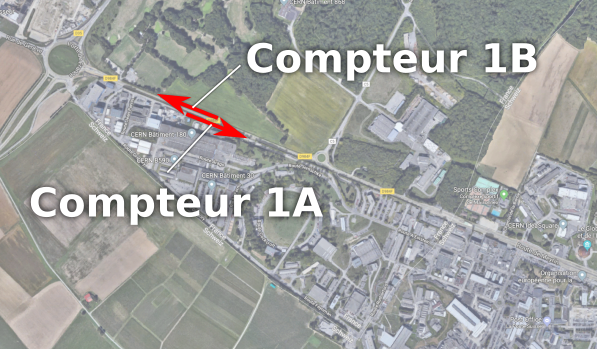
\includegraphics[width=0.35\textwidth]{images/emplacementCompteurs.png}
  \end{center}
  \vspace{-0.8cm}
  \caption{Emplacement des compteurs}
  \label{imgCompteurs}
\end{wrapfigure}

Une autre donnée pertinente est le débit de véhicules sur l'axe central reliant Genève et la France (route de Meyrin et D984). La figure \ref{imgCompteurs} montre l'emplacement des compteurs. Ceux-ci relèvent le nombre de véhicules étant passés par tranche de 15 minutes.

Le compteur nommé 1A relève donc le débit de véhicules venant de France en direction de Genève, tandis que le compteur 1B relève le débit opposé.

\newpage

\section{Résultats de l'étude}

\subsection{Introduction}

Notre simulation est dans une phase critique, autrement dit un équilibre instable. Ceci signifie qu'une petite variation dans la génération des véhicules peut se traduire par une grande augmentation du nombre de véhicules embouteillés. Cet effet est souvent appelé ``effet papillon''. Comme nous allons le voir dans les résultats, nous aurons parfois une augmentation très élevée du temps de trajet moyen ou du nombre de véhicules embouteillés sur certaines routes. Ceci n'est donc pas un effet anormal de la simulation, mais montre bien que le réseau est dans une phase d'équilibre fragile.

\subsection{Reports}

\subsubsection{Durée moyenne des trajets}

\begin{figure}[!h]
  \begin{center}
    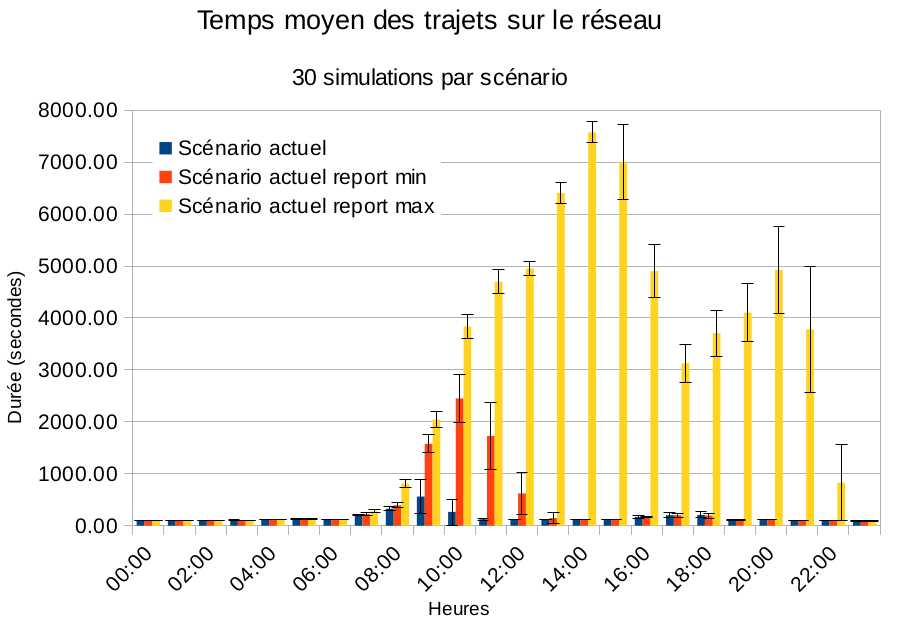
\includegraphics[width=13cm]{graphiques/temps_scenario1.png}
  \end{center}
  \vspace{-0.8cm}
  \caption{Temps moyen, scénario 1}
  \label{graphTemps1}
\end{figure}

\begin{comment}
\begin{figure}
\centering
\begin{minipage}{.5\textwidth}
  \centering
  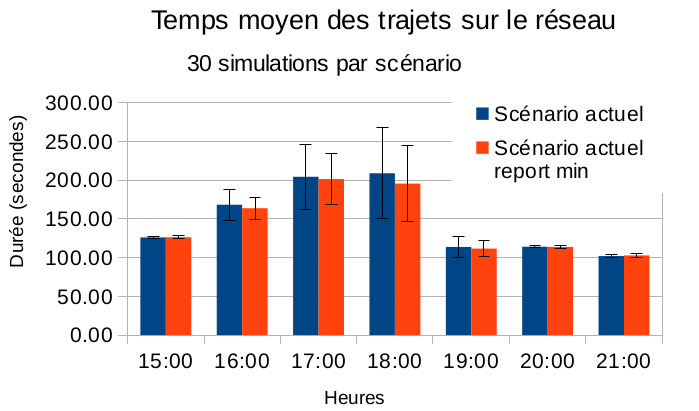
\includegraphics[width=8cm]{graphiques/temps_scenario1_zoom.png}
  \captionof{figure}{Temps moyen, scénario 1, zoom}
  \label{graphTemps1A}
\end{minipage}%
\begin{minipage}{.5\textwidth}
  \centering
  \includegraphics[width=8cm]{graphiques/temps_scenario2_zoom.png}
  \captionof{figure}{Temps moyen, scénario 2, zoom}
  \label{graphTemps1B}
\end{minipage}
\end{figure}\end{comment}

\begin{wrapfigure}[15]{r}{10cm}
  \begin{center}
    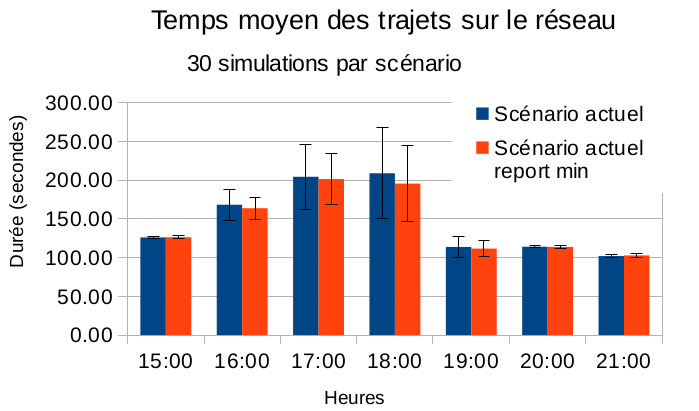
\includegraphics[width=9cm]{graphiques/temps_scenario1_zoom.png}
  \end{center}
  \caption{Temps moyen, scénario 1, zoom}
  \label{graphTemps1Zoom}
\end{wrapfigure}

Intéressons-nous tout d'abord à l'impact du report de véhicules entre les entrées A et B, et l'entrée E. Si nous regardons les résultats présentés en figure \ref{graphTemps1}, nous observons clairement que le temps moyen des trajets augmente déjà significativement pour un petit report. Dans le cas d'un grand report, nous voyons que le temps augmente grandement, à tel point que le réseau reste surchargé jusqu'à la fin de la journée. Nous voyons donc ici que ce report ne marche pas, en terme de temps de trajet moyen. Nous remarquons également sur ce graphique que l'erreur est faible, et que l'augmentation de la moyenne est bien plus élevée que la-dite erreur.

\newpage

Sur ce graphique, nous voyons clairement que l'impact d'un report minimum et maximum le matin n'est pas bénéfique. Concernant les heures de pointes du soir, nous voyons un zoom sur cette période présenté en figure \ref{graphTemps1Zoom}. Celui-ci ne présente pas le report maximum, que nous savons déjà trop élevé. Sur ce graphique, nous voyons que le report minimum aux heures de pointe du soir semble améliorer légèrement la situation. Toutefois, l'erreur étant élevée, il n'est pas garantit que cette amélioration soit certaine.

\vspace{0.4cm}

Comme nous allons le voir dans la suite de cette étude, le report des entrées A et B vers l'entrée E possède un puissant impact négatif, car le point le plus sensible du réseau se situe à l'entrée E. En effet, le temps de contrôle de cette entrée étant limité (et donc aussi le débit de cette entrée), toute modification qui augmenterait le débit vers cette entrée, ou qui augmenterait le temps nécessaire au contrôle des véhicules, viendra nécessairement créer des embouteillages sur les routes adjacentes. En ayant en tête ce point critique du système, nous comprenons aisément que reporter des véhicules vers l'entrée E aura forcément un impact négatif, éventuellement très marqué.

\subsubsection{Débit sur l'axe central}

\begin{figure}[!h]
  \begin{center}
    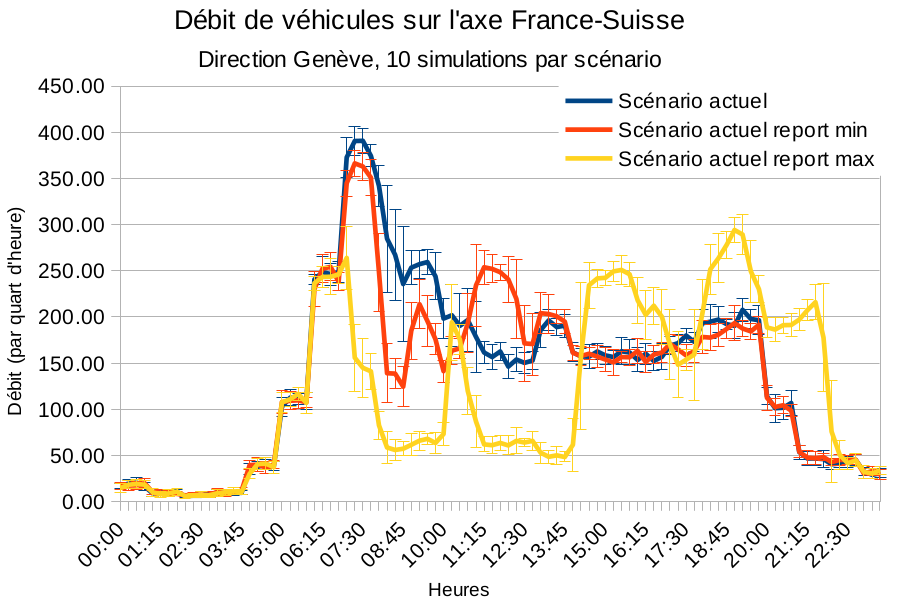
\includegraphics[width=13cm]{graphiques/compteur_1a.png}
  \end{center}
  \vspace{-0.8cm}
  \caption{Débit moyen, scénario 1}
  \label{graphCompteur1A}
\end{figure}

Si nous nous penchons maintenant sur le débit sur l'axe central (figure \ref{graphCompteur1A}), nous observons que le maximum de débit est atteint par le scénario actuel. Dans le cas du report minimum, celui-ci diminue le débit entre 8h et 11h, tandis qu'il augmente ce même débit de 11h à 14h. Ceci est en fait dû à la saturation créée le matin, qui finit par se débloquer dès 10h. Aucune amélioration n'est donc à noter pour ce report. En revanche pour le report maximum, nous voyons que dès l'heure de pointe du matin, aux alentours de 7h30, le débit chute brutalement et ne reviendra à la normale qu'aux environs de 15h. Ceci signifie donc que le réseau sature à partir de 7h30, les véhicules ne pouvant plus avancer à vitesse maximum sur l'axe central. Cette saturation continue de se maintenir jusqu'à l'après-midi (aux alentours de 14h), moment à partir duquel la saturation retombe, et les véhicules peuvent à nouveau circuler à pleine vitesse. Ceci explique donc l'apparente augmentation de débit dans le cas du report maximum dès 14h. Là encore, l'erreur est trop faible pour mettre en doute les conclusions que nous pouvons en tirer. 

\vspace{0.4cm}

À noter également les paliers, qui sont particulièrement visible sur les heures du matin, entre minuit et 7h. Ceci est dû au fait que les données initiales que nous avons reçues sont horaires, signifiant donc que la génération de véhicules est constante au sein d'une même heure. 

\newpage

\subsubsection{Taille des files de véhicules}

\begin{figure}[!h]
  \begin{center}
    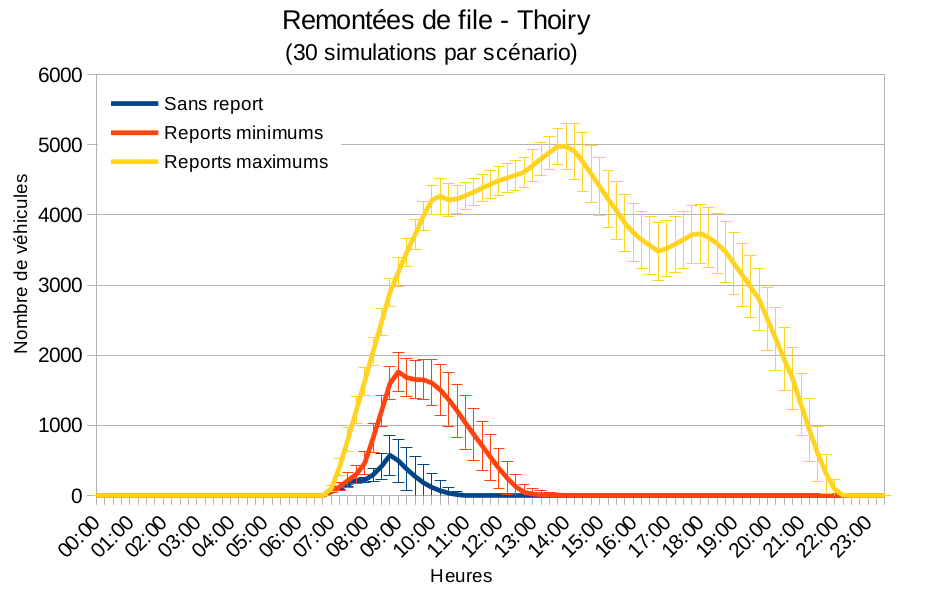
\includegraphics[width=12cm]{graphiques/leakyB_thoiry_scenario1.png}
  \end{center}
  \vspace{-0.8cm}
  \caption{Taille des files, Thoiry}
  \label{graphLBThoiry}
\end{figure}

Observons tout d'abord la remontée de véhicules sur la route venant de Thoiry (D884). La figure \ref{graphLBThoiry} présente la taille de la file venant de Thoiry. Nous voyons que le report minimum crée une augmentation significative du nombre de véhicules embouteillés. Alors que nous avions initialement une remontée de file d'environ 500 véhicules en moyenne sur cette route aux heures de pointe du matin sans faire de report, cette remontée monte jusqu'à 1800 véhicules pour une report minimum, et jusqu'à 5000 pour un report maximum. Cette augmentation dépasse largement l'erreur, ce qui signifie que cet effet est garantit. Dans le cas d'un report maximum, la magnitude de cet effet augmente à tel point qu'il faut presque la journée entière pour que cette file de véhicule se résorbe. 

\begin{figure}[!h]
  \begin{center}
    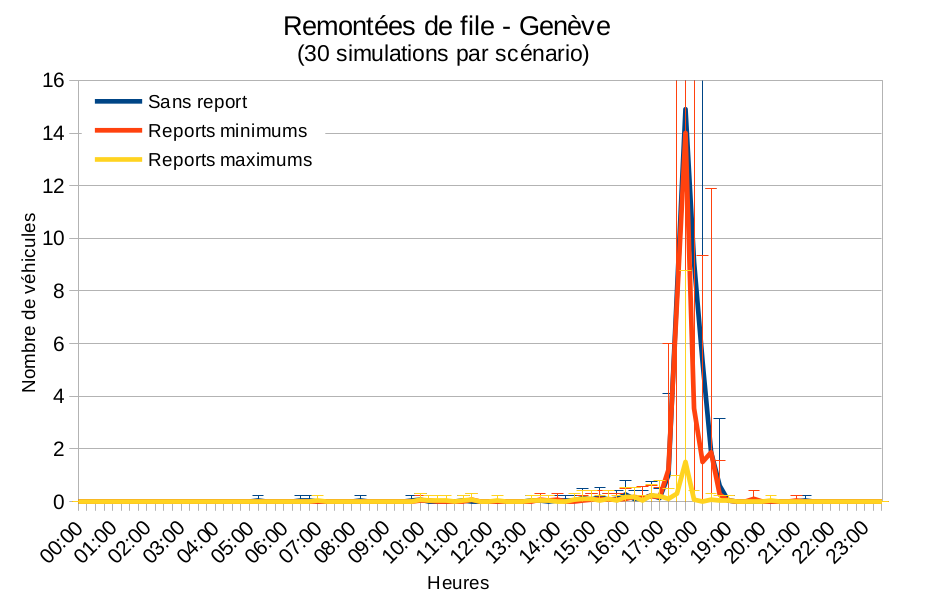
\includegraphics[width=12cm]{graphiques/leakyB_geneve_s1.png}
  \end{center}
  \vspace{-0.8cm}
  \caption{Taille des files, Genève}
  \label{graphLBGeneve}
\end{figure}

Nous pouvons également observer la taille de la file de véhicules venant de Genève, sur la route de Meyrin. La figure \ref{graphLBGeneve} présente ces données. Comme nous le voyons avec l'axe vertical, la taille de cette file est en effet très restreinte. Le maximum de cette file ne dépasse pas vingt véhicules, ce qui ne peut pas être considéré comme un réel embouteillage. Nous observons que les reports ont toutefois un impact bénéfique sur la route de Meyrin en venant de Genève, et sur les heures de pointes du soir uniquement, bien que celui-ci ne soit appliquer qu'à une vingtaine de véhicules.

\newpage

\subsection{Scénario 2 et reports}

Passons maintenant au scénario 2 (rond-point à la place du carrefour de l'entrée B), tout en conjuguant ce scénario avec les reports que nous avons testés précédemment. Il est en effet possible que les reports soient bénéfiques mais uniquement dans ce scénario-ci.

\subsubsection{Durée moyenne des trajets}

\begin{figure}[!h]
  \begin{center}
    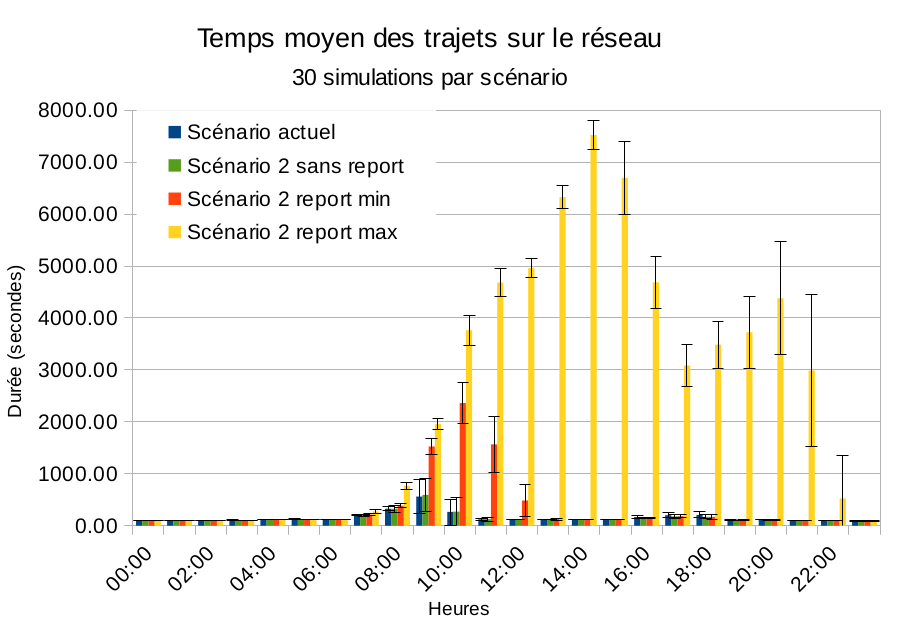
\includegraphics[width=13cm]{graphiques/temps_scenario2.png}
  \end{center}
  \vspace{-0.8cm}
  \caption{Temps moyen, scénario 2}
  \label{graphTemps2}
\end{figure}

\begin{wrapfigure}[17]{r}{10cm}
  \begin{center}
    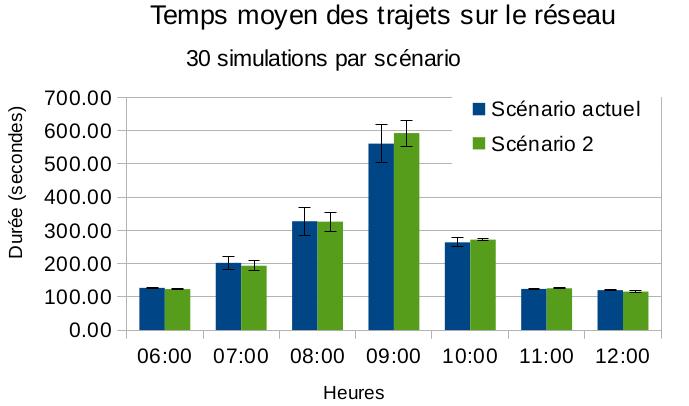
\includegraphics[width=9cm]{graphiques/temps_scenario2_zoom1.png}
  \end{center}
  \caption{Temps moyen, scénario 2, zoom HPM}
  \label{graphTemps2Zoom1}
\end{wrapfigure}

Intéressons-nous maintenant au scénario d'un rond-point à la place du carrefour de l'entrée B. Comme précédemment nous remarquons que le report de véhicule, même dans le cas du scénario 2, empire la situation actuelle en terme de temps moyen passé sur le réseau. A nouveau, il est bien plus intéressant de se concentrer sur les scénarios sans report. La figure \ref{graphTemps2Zoom1} présente l'heure de pointe pour ces deux scénarios. Comme nous le voyons, le scénario actuel semble être légèrement meilleur que le scénario du rond-point à ces heures de la journée. En revanche, l'erreur est trop élevée en regard de la différence entre les deux courbes. C'est pourquoi il nous n'est pas possible d'affirmer de manière sûre que le scénario actuel soit meilleur pour les heures de pointe du matin.

\newpage

\begin{wrapfigure}[9]{r}{10cm}
  \begin{center}
    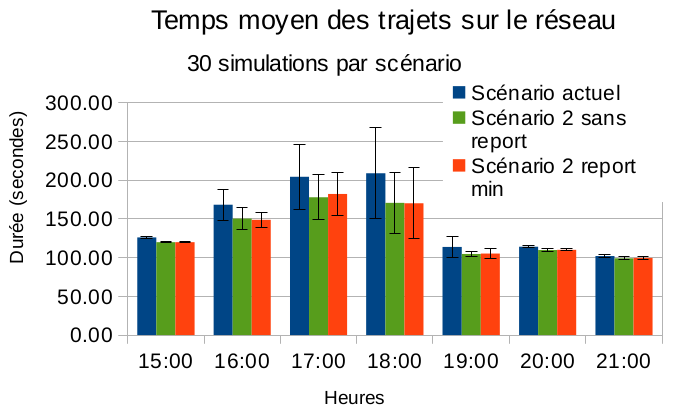
\includegraphics[width=9cm]{graphiques/temps_scenario2_zoom2.png}
  \end{center}
  \caption{Temps moyen, scénario 2, zoom HPS}
  \label{graphTemps2Zoom2}
\end{wrapfigure}

Si nous observons maintenant les heures de pointe du soir (figure \ref{graphTemps2Zoom2}), nous voyons que la situation est différente. Le report minimum n'a quasiment aucun impact, alors que le rond-point améliore la situation, malgré une erreur relativement élevée. Il semble donc que le rond-point soit spécialement bénéfique le soir. Celui-ci améliore le temps moyen des trajets entre 10 et 20$\%$.

\vspace{2cm}

\subsubsection{Débit sur l'axe central}

\begin{figure}[!h]
  \begin{center}
    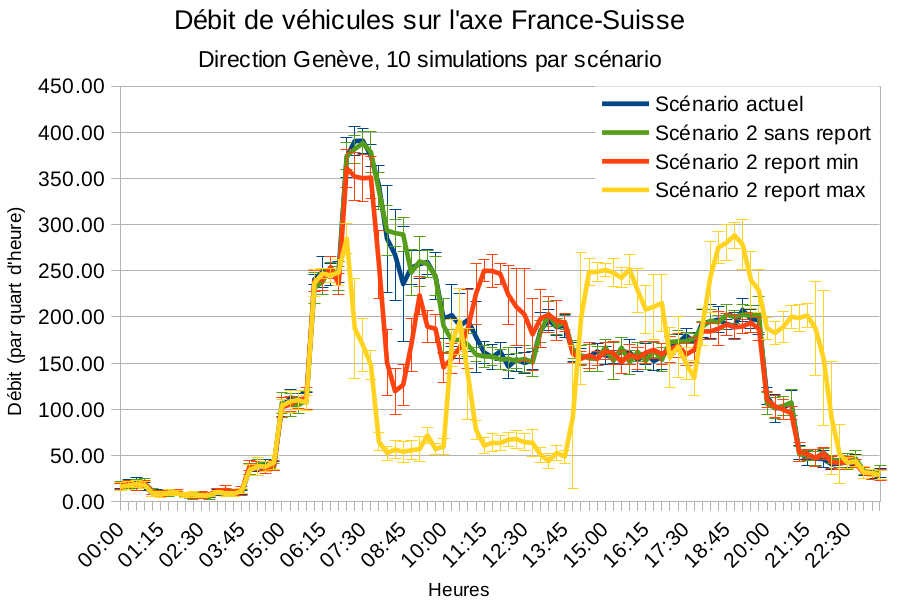
\includegraphics[width=13cm]{graphiques/compteur_1a_scenario2.png}
  \end{center}
  \vspace{-0.8cm}
  \caption{Débit moyen, direction Genève, scénario 2}
  \label{graphCompteur1AScenario2}
\end{figure}

Pour ce qui est du débit sur l'axe central, il est clair que le scénario 2 ne crée que quelques maigres variations sur le débit moyen, qui ne sont pas significatives. De même que pour précédemment le report, bien qu'appliqué cette fois au scénario 2, n'a pas un bon impact sur le réseau.

\subsubsection{Taille des files de véhicules}

\begin{figure}[!h]
  \begin{center}
    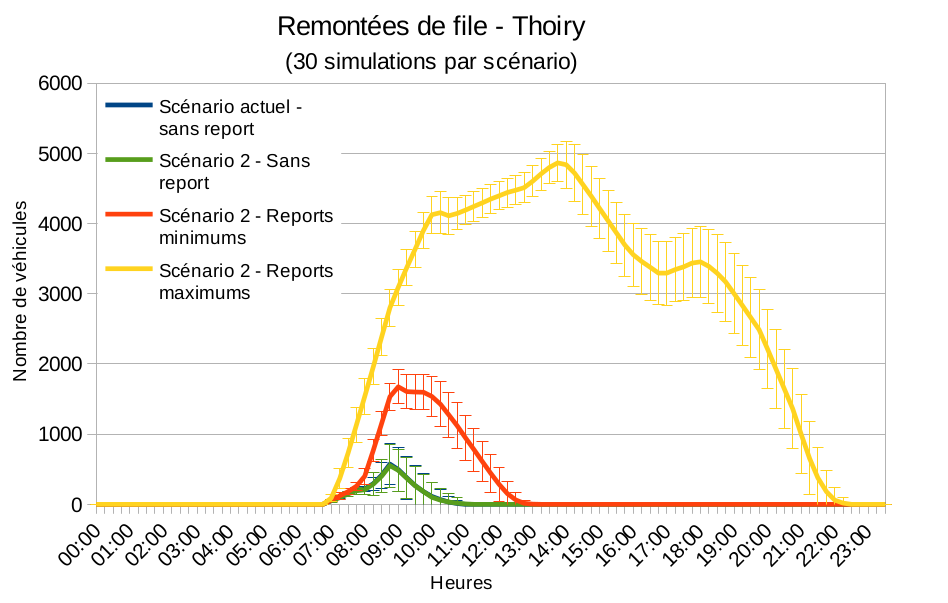
\includegraphics[width=13cm]{graphiques/leakyB_thoiry_s2.png}
  \end{center}
  \vspace{-0.8cm}
  \caption{Taille des files, Thoiry, scénario 2}
  \label{graphLBThoiryS2}
\end{figure}

La figure \ref{graphLBThoiryS2} présente la taille de la file venant de Thoiry, pour le scénario 2 avec et sans report, en comparaison du scénario actuel. Comme précédemment, l'impact du report est très négatif, avec les mêmes valeurs que dans le scénario initial. Nous voyons également que le scénario 2 sans report ne semble pas avoir d'impact sur cette file de véhicules. Regardons plus en détail le scénario actuel et le scénario 2 sur les heures de pointe du matin (figure \ref{graphLBThoiryS2Zoom}). Comme nous pouvons le voir, les deux scénarios ne modifient pas la taille de la file, la différence entre les deux étant très petite par rapport à l'erreur. En conclusion, le scénario 2 n'améliore pas de manière significative la taille de cette file de véhicules.

\begin{figure}[!h]
  \begin{center}
    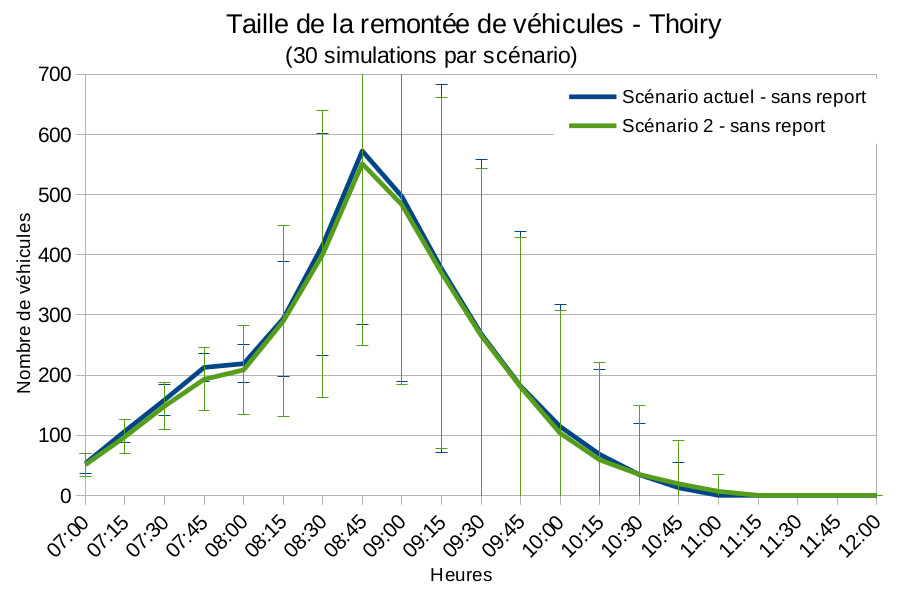
\includegraphics[width=8cm]{graphiques/leakyB_thoiry_s1s2.png}
  \end{center}
  \vspace{-0.8cm}
  \caption{Taille des files, Thoiry, scénario 2, zoom}
  \label{graphLBThoiryS2Zoom}
\end{figure}

\begin{figure}[!h]
  \begin{center}
    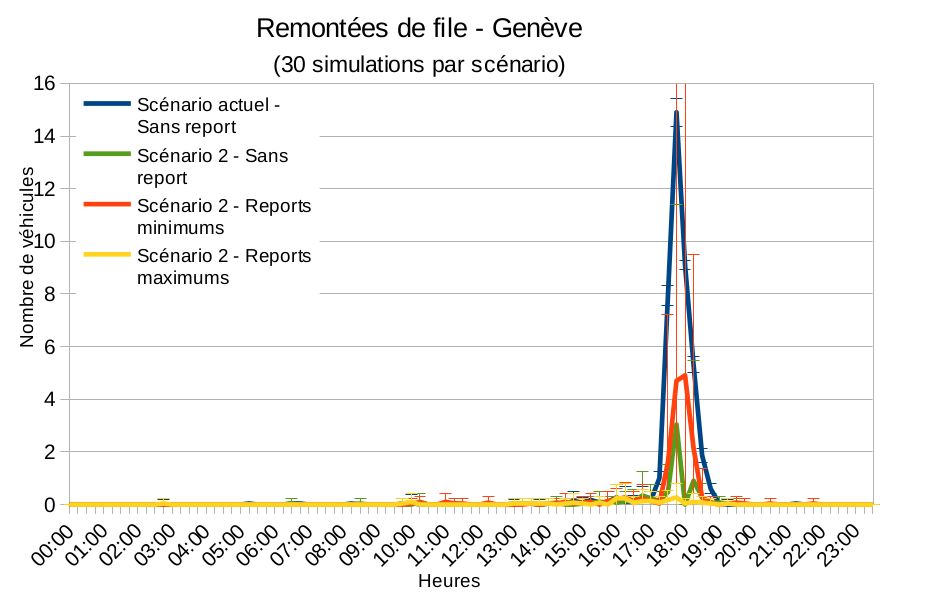
\includegraphics[width=13cm]{graphiques/leakyB_geneve_s2.png}
  \end{center}
  \vspace{-0.8cm}
  \caption{Taille des files, Genève, scénario 2}
  \label{graphLBGeneveS2}
\end{figure}

Dans le cas de la file de véhicules sur la route de Meyrin (figure \ref{graphLBGeneveS2}, nous observons que le meilleur scénario est la conjugaison du scénario 2 avec report maximum. Mais au vu de l'erreur importante (dûe au nombre de véhicules dans cet file), cette amélioration apparente ne peut pas être garantie. Toutefois, de part son erreur plus faible, le report maximum semble en effet apporter une amélioration.

\newpage

\subsection{Entrée E}

\subsubsection{Durée moyenne des trajets}

\begin{figure}[!h]
  \begin{center}
    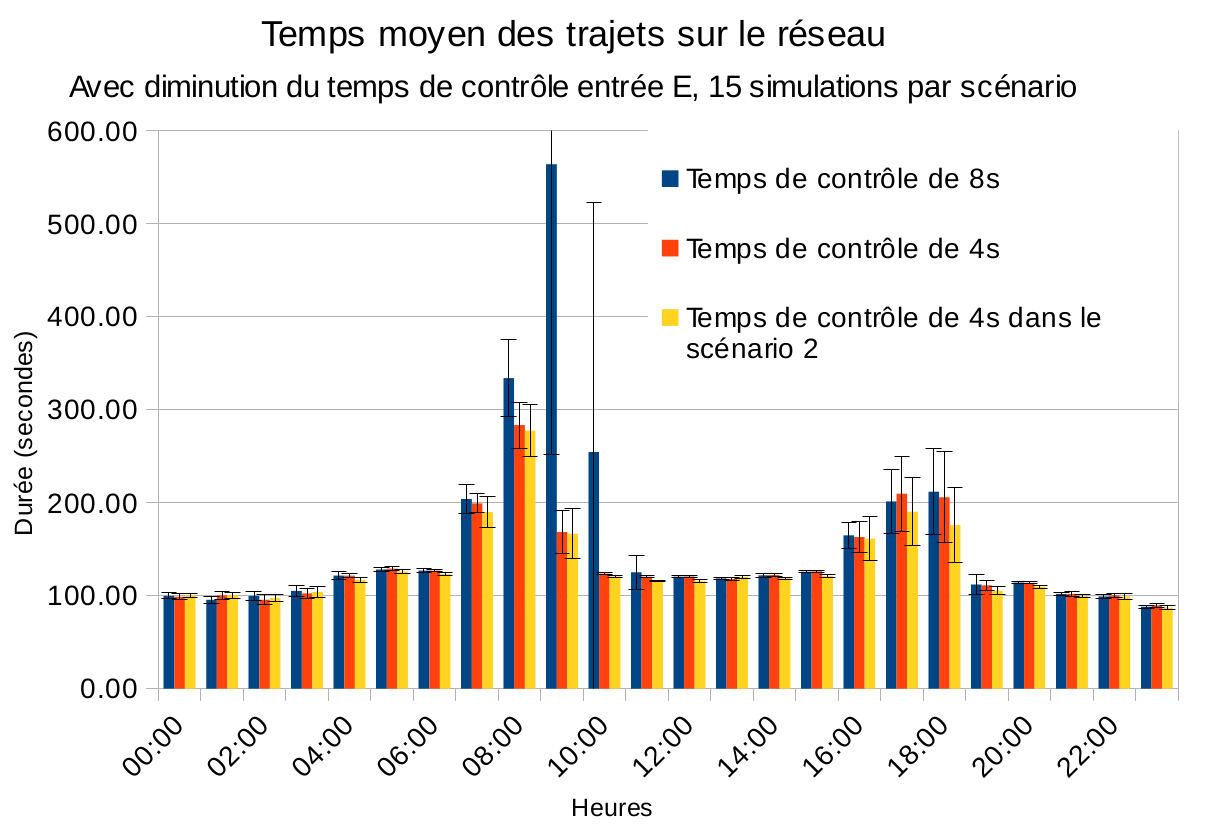
\includegraphics[width=13cm]{graphiques/temps_entreeE.png}
  \end{center}
  \vspace{-0.8cm}
  \caption{Temps moyen, scénario entrée E}
  \label{graphTempsE}
\end{figure}

Finalement, le dernier scénario que nous allons étudier sera celui d'une entrée E permettant un contrôle plus rapide des véhicules, et donc un débit plus élevé. Comme nous le voyons sur la figure \ref{graphTempsE}, la durée des contrôles à l'entrée E a un grand impact sur la durée des trajets sur le réseau. En effet, pour une durée de contrôle passant de 8 secondes à 4 secondes, le temps moyen diminue largement, jusqu'à diminuer de près de trois fois pour la plage horaire de 9h à 10h. Sur le scénario initial, nous percevons clairement que la saturation aux heures de pointe du matin se reporte sur les heures suivantes, expliquant que le maximum se situe à 9h. En revanche, dans le scénario d'une entrée E avec un meilleur débit, nous voyons clairement que cette saturation se résorbe bien plus rapidement, le temps moyen atteignant son sommet à 8h. Au vu des marges d'erreur, nous pouvons sans doute affirmer que l'entrée E est le meilleur scénario que nous avons étudié jusque là.

\vspace{0.4cm}

Aux heures de pointe du soir, un changement dans le débit de l'entrée E n'a pas d'impact notable, comme nous pouvons nous y attendre.

\subsubsection{Débit sur l'axe central}

\begin{figure}[!h]
  \begin{center}
    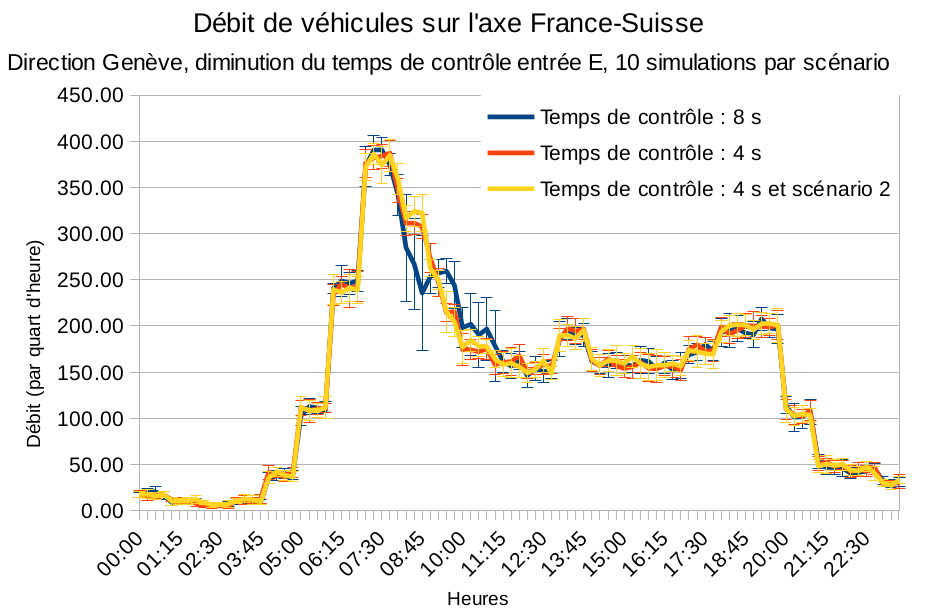
\includegraphics[width=13cm]{graphiques/compteur_1a_entreeE.png}
  \end{center}
  \vspace{-0.8cm}
  \caption{Débit moyen, direction Genève, scénario entrée E}
  \label{graphCompteur1AScenarioE}
\end{figure}

De la même manière, un changement dans le temps de contrôle à l'entrée E n'a aucun impact sur le débit de l'axe central. Un léger impact se fait ressentir aux alentours de 8h, mais globalement l'impact reste très limité.

\newpage

\subsubsection{Taille des files de véhicules}

\begin{figure}[!h]
  \begin{center}
    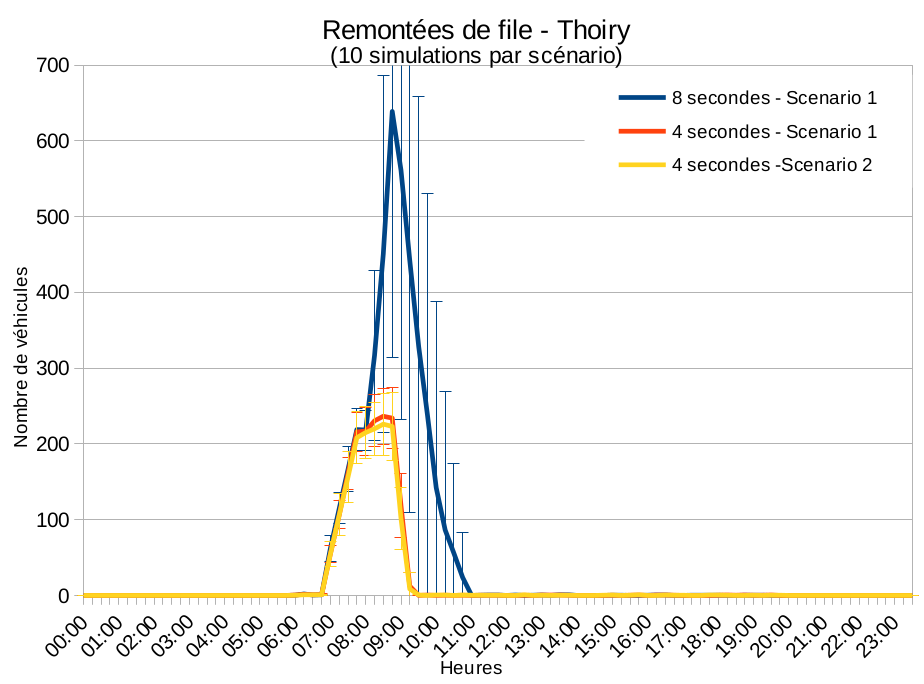
\includegraphics[width=13cm]{graphiques/leakyB_entreeE.png}
  \end{center}
  \vspace{-0.8cm}
  \caption{Taille des files, Thoiry, scénario entrée E}
  \label{graphLBThoirySE}
\end{figure}

Dans la continuité des précédentes mesures, nous voyons que l'entrée E réduit grandement la taille de cette file de véhicules. Nous passons en effet d'environ 640 véhicules embouteillés à 240 véhicules. Cette amélioration est donc tout à fait significative, d'autant plus que l'erreur est faible en regard de la diminution observée.

\vspace{0.4cm}

En conclusion de ce dernier scénario, nous avons clairement mis en évidence qu'il améliore non seulement la file de véhicules de Thoiry, mais également le temps moyen que passent les véhicules sur le réseau. Ce scénario est donc le meilleur que nous avons à proposer dans cette étude.

\begin{comment}
\begin{figure}[!h]
  \begin{center}
    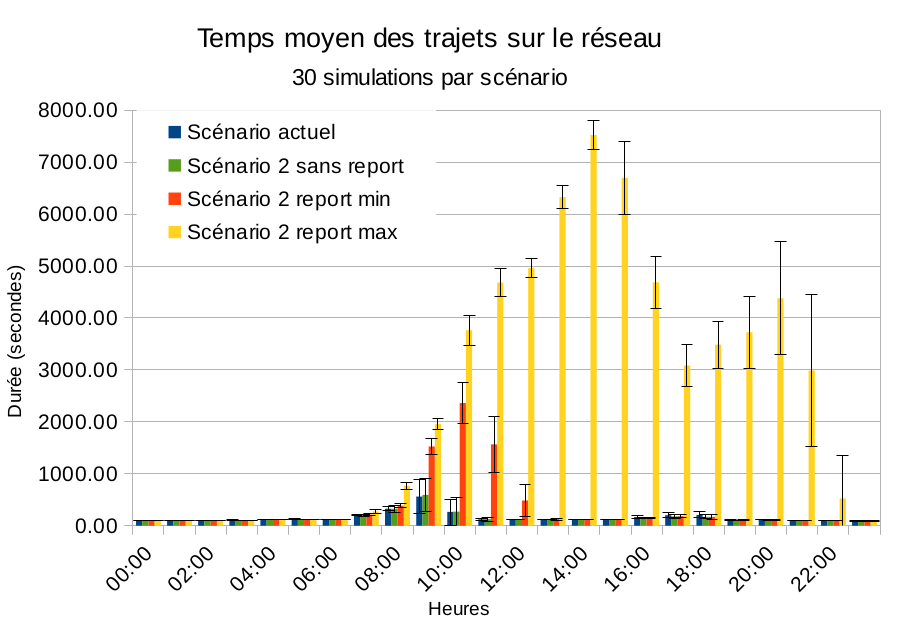
\includegraphics[width=14cm]{graphiques/temps_scenario2.png}
  \end{center}
  \vspace{-0.8cm}
  \caption{Temps moyen, scénario 2}
  \label{graphTemps2}
\end{figure}

\begin{figure}[!h]
  \begin{center}
    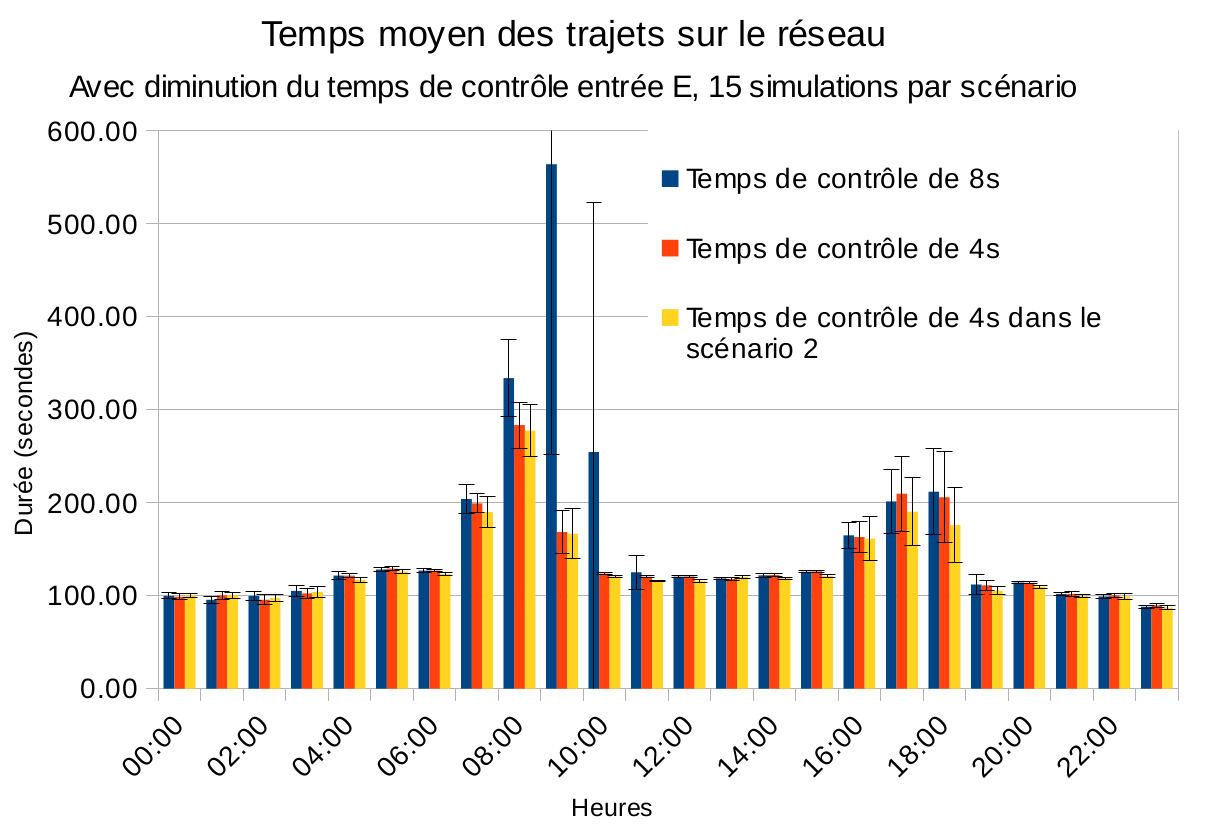
\includegraphics[width=14cm]{graphiques/temps_entreeE.png}
  \end{center}
  \vspace{-0.8cm}
  \caption{Temps moyen, contrôle entrée E plus rapide}
  \label{graphTemps2}
\end{figure}\end{comment}

\newpage

\section{Conclusion}

Comme nous l'avons vu au travers des différentes mesures qui ont été effectuées pour ces scénarios, le report de véhicules tel que proposé actuellement a un impact négatif le matin, ainsi qu'un léger impact positif le soir. Bien que ces reports ne semblent pas avoir de réel impact positif, il est toutefois possible que d'autres types de reports puissent améliorer le trafic au CERN. Par exemple, un report inversé le matin (de l'entrée E vers les entrées A et B) pourrait s'avérer pertinent. De même, il est possible qu'un report vers le tunnel inter-site puisse améliorer la circulation. Mais dans ces deux cas, il est nécessaire d'étudier la question pour s'en assurer.

\vspace{0.4cm}

Le scénario consistant à remplacer le carrefour à feux de l'entrée B par un rond-point, a montré une légère amélioration mais uniquement le soir. Lors des heures de pointe du matin, celui-ci ne permet d'améliorer la circulation. Il est en effet assez logique qu'un rond-point à cet endroit améliore légèrement la circulation (les ronds-points étant toujours plus efficaces que des carrefours), mais étant donné que l'impact est faible, il faut se demander s'il est judicieux de procéder à de lourds travaux pour un impact aussi faible.

\vspace{0.4cm}

Finalement, une diminution du temps de contrôle à l'entrée E a montré un très grand impact positif, particulièrement sur la zone française et sur la route D884. Un tel changement améliore également le temps moyen que les véhicules passent sur le réseau. C'est donc sans nul doute le meilleur scénario que nous avons éprouvé dans cet étude.

\newpage

\appendix

\section{\label{appData}Données utilisées}

\begin{figure}[!h]
  \begin{center}
    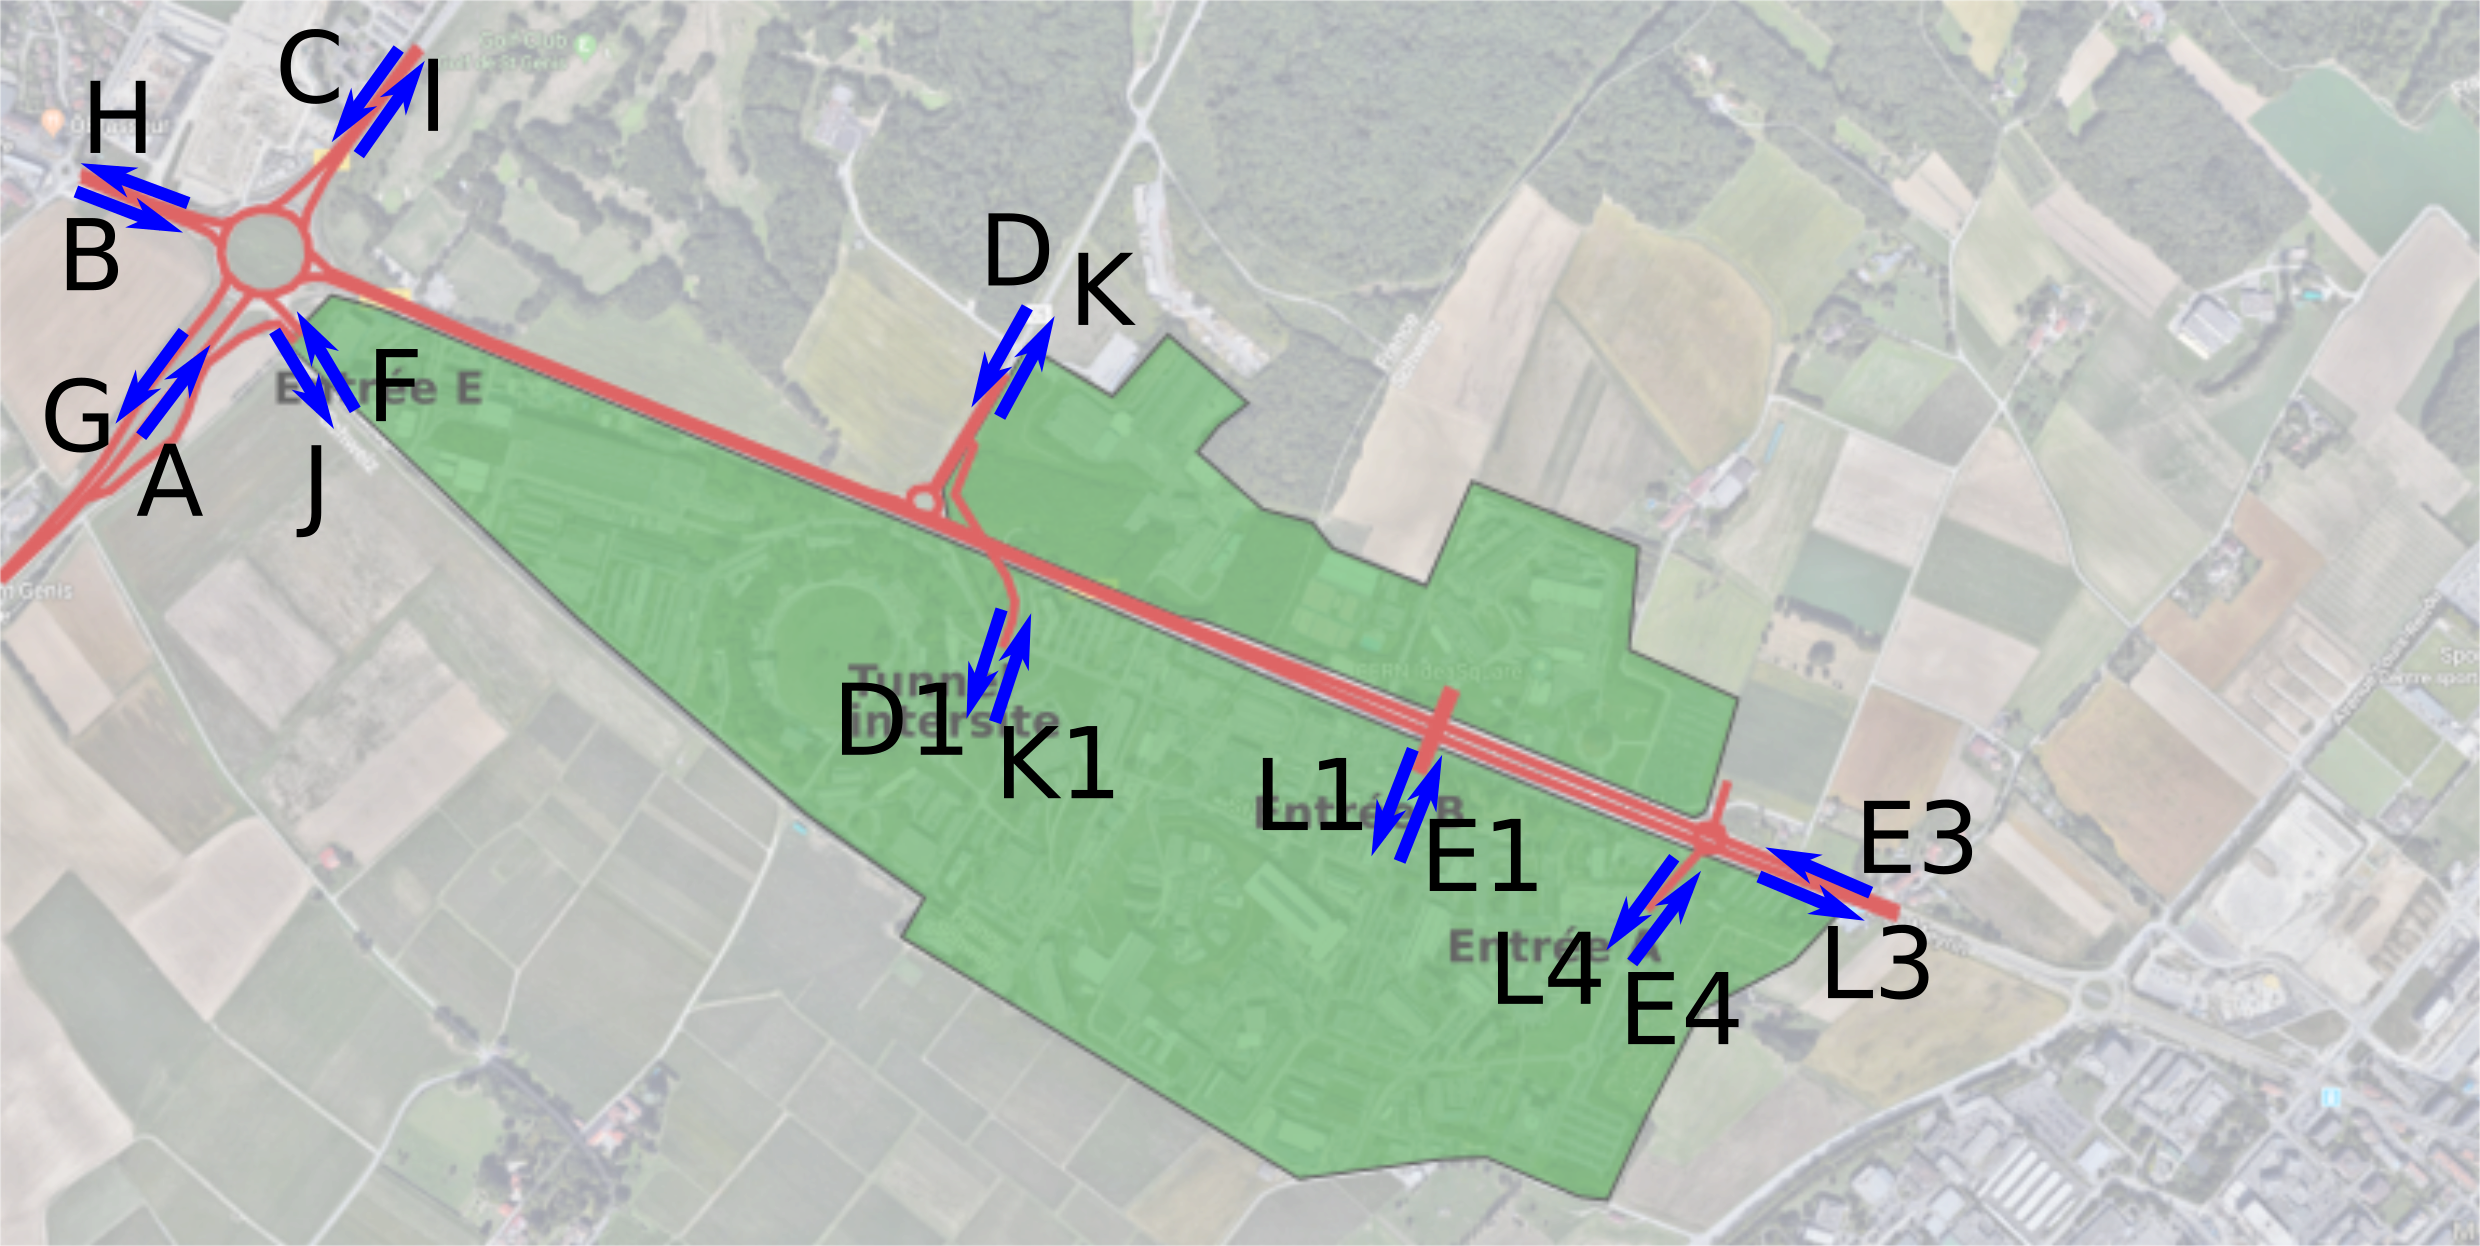
\includegraphics[width=13cm]{images/reseauNoms.png}
  \end{center}
  %\vspace{-0.8cm}
  \caption{Noms des entrées/sorties du réseau internes à la simulation, utilisés en figures \ref{imgData} et \ref{imgDataProba} (ne pas confondre avec les noms des entrées du CERN : A, B et E)}
  \label{imgNomsIO}
\end{figure}

\begin{figure}[!h]
  \begin{center}
    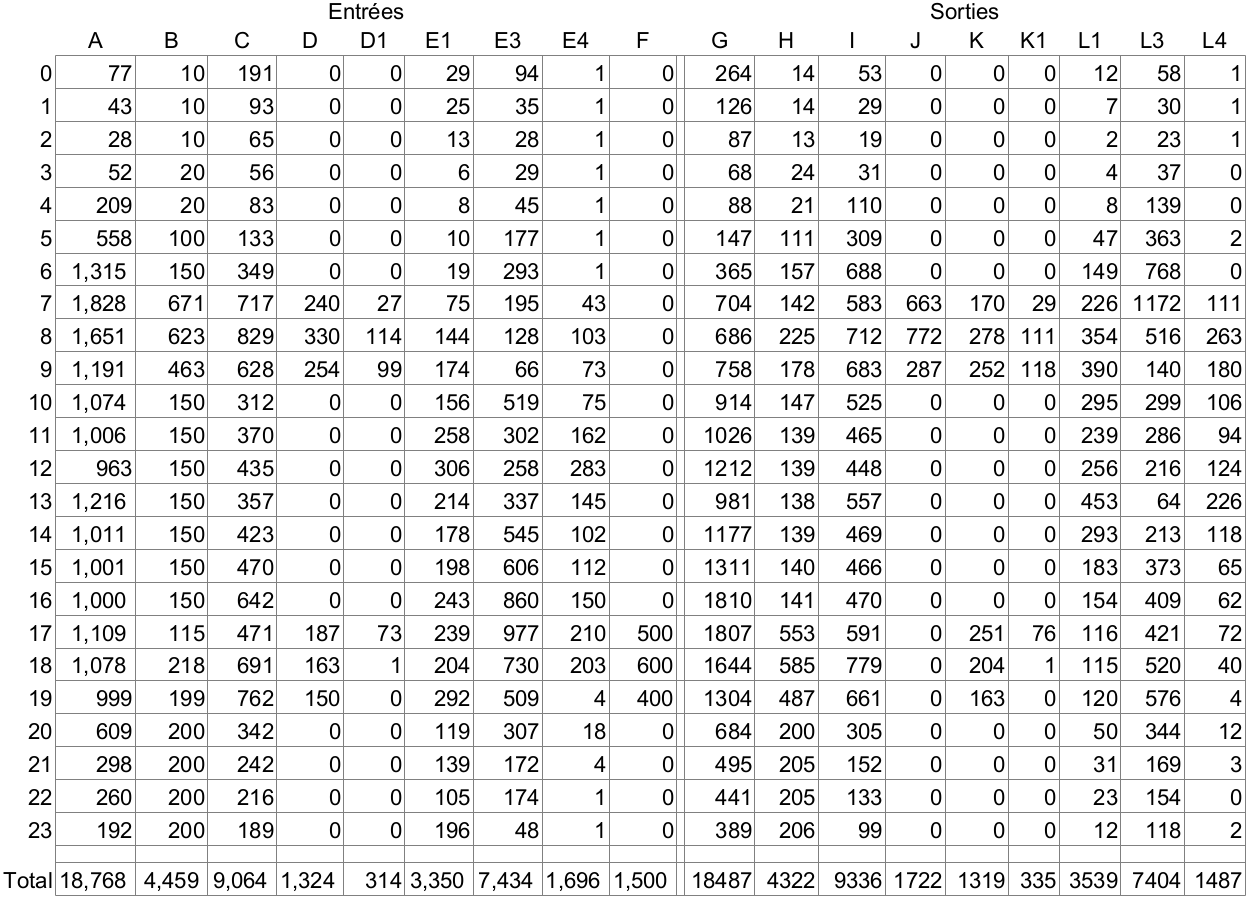
\includegraphics[width=16cm]{images/donneesInitiales.png}
  \end{center}
  %\vspace{-0.8cm}
  \caption{Données initiales utilisées, horizontalement les entrées/sorties tels que nommées en figure \ref{imgNomsIO}, verticalement les heures de la journée (ne pas confondre avec les noms des entrées du CERN : A, B et E)}
  \label{imgData}
\end{figure}

\begin{figure}[!h]
  \begin{center}
    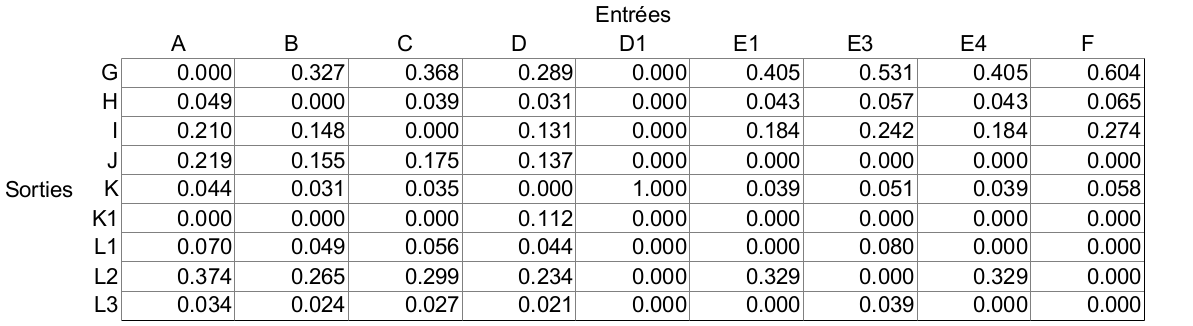
\includegraphics[width=16cm]{images/donneesInitialesProba.png}
  \end{center}
  %\vspace{-0.8cm}
  \caption{Probabilités pour la tranche horaire 7h-8h, généré d'après le tableau de la figure \ref{imgData}, horizontalement les entrées, verticalement les sorties (ne pas confondre avec les noms des entrées du CERN : A, B et E)}
  \label{imgDataProba}
\end{figure}

\section{Références}

\begin{itemize}
\item \emph{Cellular Automata Simulations of Traffic: A Model for the City of Geneva}, A. Dupuis et B. Chopard, Networks and Spatial Economics, 3: (2003) 9–21
\item Travail de thèse de Samia Smaili, Université d'Evry Val d'Essonne, janvier 2012
\item Modélisation du trafic routier par des automates cellulaires, Cécile Appert (CNRS et ENS) et Ludger Santen (Université de Saarlandes), septembre 2015
\end{itemize}

\begin{comment}

\begin{wrapfigure}[23]{r}{0.4\textwidth}
  \begin{center}
    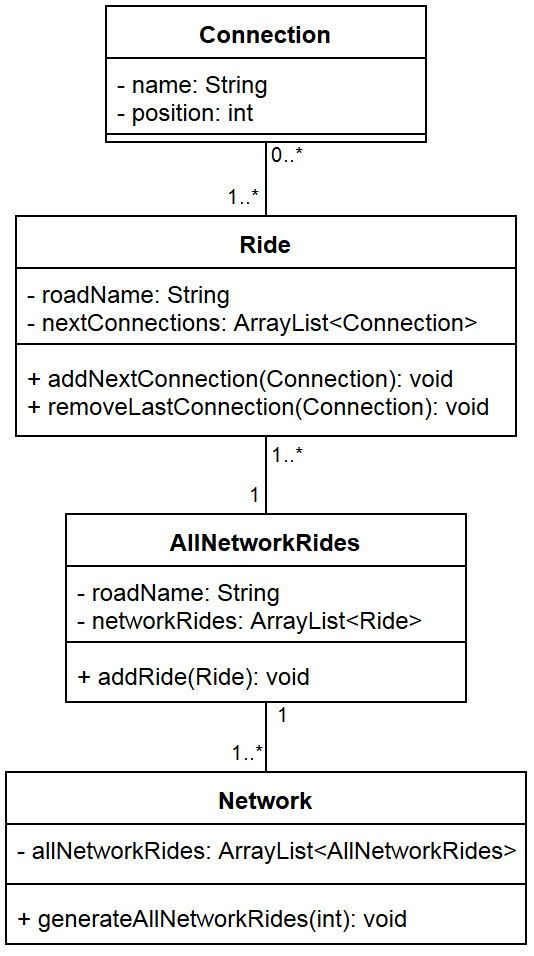
\includegraphics[width=0.35\textwidth]{rides_diagram.png}
  \end{center}
  \caption{Diagramme de classe des trajets}
  \label{imgRides}
\end{wrapfigure}

\begin{figure}[!h]
  \begin{center}
    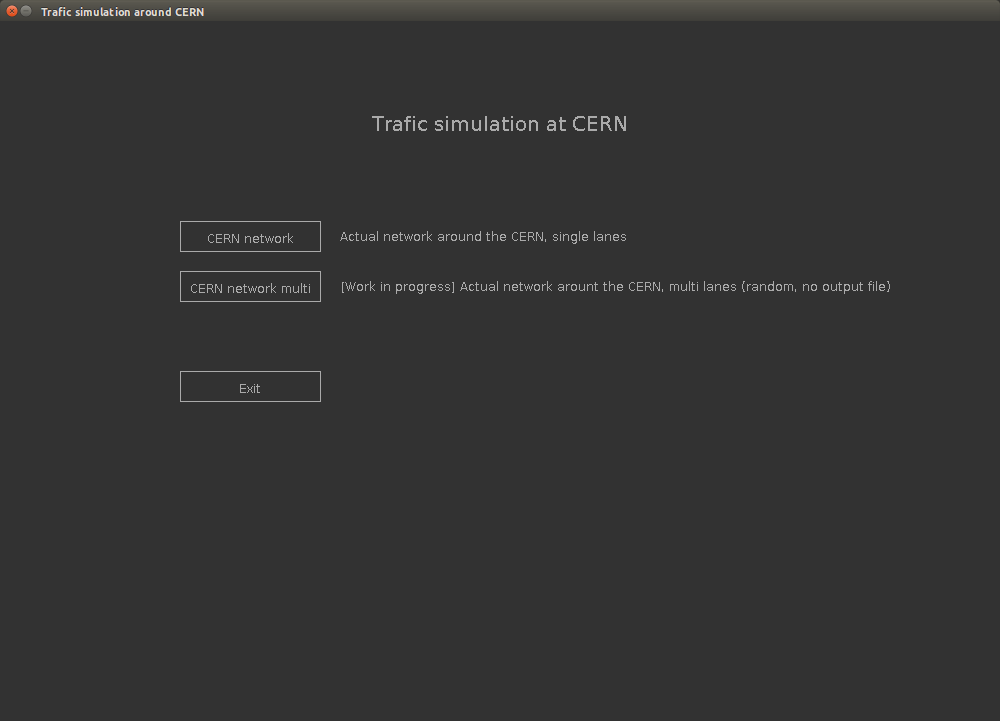
\includegraphics[width=0.7\textwidth]{interface_menu.png}
  \end{center}
  \caption{Menu du programme}
  \label{imgMenu}
\end{figure}

\end{comment}

\end{document}
